\section{Architecture}

In order to have a huge flexibility in our bot behaviors we designed our AI in a modular and hierarchical fashion (Figure \ref{classDiag}).
This architecture and the addition of behaviors tree was perfectly fitted for the development of multiple bots -- small part of the code has to be change to improve/change the bot behavior.
It also looks like a human hierarchy -- faciliting the conception of each bot.

\begin{figure}[h!t]
\centering
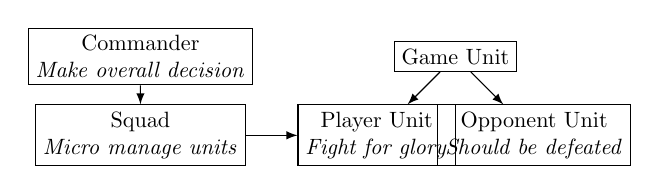
\begin{tikzpicture}[node distance = 1 cm]
    \tikzstyle{quadri}=[rectangle,draw, align=center, scale=0.8]
    \tikzstyle{link}=[->,thin,>=latex]
    \node[quadri] (commander) at (-2,2) {Commander \\ \emph{Make overall decision}};
    \node[quadri] (squad) at (-2,1) {Squad \\ \emph{Micro manage units}};
    \draw[link] (commander)--(squad);

    \node[quadri] (gameUnit) at (2,2) {Game Unit};
    \node[quadri] (pUnit) at (1,1){Player Unit \\ \emph{Fight for glory}};
    \node[quadri] (oUnit) at (3,1){Opponent Unit \\ \emph{Should be defeated}};

    \draw[link] (squad)--(pUnit);
    \draw[link] (gameUnit)--(pUnit);
    \draw[link] (gameUnit)--(oUnit);
\end{tikzpicture}
\caption{Class Diagram}
\label{classDiag}
\end{figure}

\begin{definition}[Commander, Squad, Units]
    \ \\
    \begin{description}
        \item[Commander:]  One per game who make overall decision for the game such as: Creating squad, assigning objectives to squads (\texttt{Attack}, \texttt{Flee}, \texttt{Go to}, \ldots).
        \item[Squad:] As many squad as the commander want. They have a military goal and are in charge of micro-managing each units. 
        \item[Unit:] Each game unit has many attributes and some scripted behaviors (\texttt{Attack closest ennemy}, \texttt{Regroup with squad}, \texttt{Attack ennemy with kitting strategy}, \ldots)
    \end{description}
\end{definition}

